% =====================================================================
% Semana 1 · S1.4 — Potencia nominal y derating
% Fundamentos de Sistemas Electrónicos Analógicos (Ingeniería Aeroespacial)
% Compilar: pdflatex semana_1_s14_potencia_derating.tex  (2 pasadas)
% =====================================================================
\documentclass[aspectratio=169]{beamer}

\usepackage[utf8]{inputenc}
\usepackage[T1]{fontenc}
\usepackage{lmodern}
\usepackage[spanish,es-tabla]{babel}
\usepackage{amsmath,amssymb}
\usepackage{siunitx}
\usepackage{booktabs}
\usepackage{microtype}
\usepackage{circuitikz}

\definecolor{navy}{RGB}{23,54,93}
\definecolor{navysoft}{RGB}{72,101,140}
\definecolor{gold}{RGB}{179,142,62}
\definecolor{ink}{RGB}{44,51,58}
\definecolor{soft}{RGB}{244,241,234}

\usetheme{default}
\setbeamertemplate{navigation symbols}{}
\setbeamertemplate{footline}[frame number]
\setbeamercolor{structure}{fg=navy}
\setbeamercolor{frametitle}{fg=white,bg=navy}
\setbeamercolor{title}{fg=navy}
\setbeamercolor{subtitle}{fg=navysoft}
\setbeamercolor{itemize item}{fg=gold}
\setbeamercolor{itemize subitem}{fg=gold}
\setbeamercolor{block title}{fg=white,bg=navy}
\setbeamercolor{block body}{bg=soft}
\setbeamercolor{example text}{fg=navy}
\setbeamertemplate{itemize item}{\scriptsize\raise1.25pt\hbox{\donotcoloroutermaths$\bullet$}}
\setbeamertemplate{itemize subitem}{\scriptsize\raise1.25pt\hbox{\donotcoloroutermaths$\circ$}}
\setbeamerfont{frametitle}{size=\large,series=\bfseries}

\title[S1.4 · Derating]{Potencia nominal y derating}
\subtitle{S1.4 — Simulaciones y laboratorio de la Semana 1}
\institute{Licenciatura en Ingeniería Aeroespacial\\ UNAM · ENES Unidad Juriquilla}
\author{M. en C. José de Jesús Santana Ramírez}
\date{Semestre 2027-1}

\begin{document}

% ---------------------------------------------------------------------
\begin{frame}[plain]
  \titlepage
\end{frame}

% ---------------------------------------------------------------------
\begin{frame}{Objetivos de la sesión}
  \begin{itemize}
    \item Interpretar la \textbf{potencia nominal} de un resistor ($P_{nominal}$) y su significado físico.
    \item Aplicar la regla de \textbf{derating de 50\,\%} y calcular el límite de diseño.
    \item Determinar \textbf{a qué tensión} un resistor de $1\,\text{k}\Omega$ / \SI{0.25}{\watt} alcanza su límite.
    \item Conectar el resultado con el \textbf{barrido de S1.1} (la potencia crece con $V^2$).
    \item Decidir con criterio de diseño: \emph{aceptado, condicionado o rechazado}.
  \end{itemize}
  \pause
  \begin{block}{Pregunta rectora del curso}
    Un resistor que ``funciona'' en el cálculo básico, ¿sobrevivirá diez años en órbita sin convección, con vibración y ciclos térmicos?
  \end{block}
\end{frame}

% ---------------------------------------------------------------------
\begin{frame}{Teoría 1 · ¿Qué significa \SI{0.25}{\watt}?}
  \begin{itemize}
    \item La \textbf{potencia nominal} es la máxima potencia que el componente puede disipar
      \emph{de forma continua} sin exceder su temperatura máxima de operación.
    \item Se especifica a una temperatura ambiente (típicamente \SI{70}{\celsius} para resistores de carbón/metal).
    \item La disipación es efecto Joule: el resistor convierte energía eléctrica en \textbf{calor}.
  \end{itemize}
  \[
    P_{disipada} = V\cdot I = I^2\,R = \frac{V^2}{R}
  \]
  \pause
  \begin{itemize}
    \item Con $R$ fija, la potencia crece con el \textbf{cuadrado} de la tensión:
      subir de 12 V a 14 V aumenta la disipación un 36\,\%.
    \item El resistor ``no se entera'' de cuánto puede disipar: se calienta y falla si el calor no se evacúa.
  \end{itemize}
\end{frame}

% ---------------------------------------------------------------------
\begin{frame}{Teoría 2 · Derating: operar por debajo del límite}
  \begin{block}{Definición}
    El \textbf{derating} consiste en operar los componentes por debajo de sus límites
    máximos declarados para reducir la tasa de falla y compensar variaciones ambientales.
  \end{block}
  \pause
  \begin{itemize}
    \item Regla práctica para resistores: $\;P_{disipada} \le 0.5\cdot P_{nominal}$.
    \item Compensa: envejecimiento, ciclos térmicos, radiación, tolerancias y el \textbf{vacío} (sin convección).
    \item Estándares rectores: \textbf{NASA EEE-INST-002} y \textbf{ECSS-Q-ST-30-11C} (derating del 50\,\% para resistores); respaldo en NASA LLIS-0676.
  \end{itemize}
\end{frame}

% ---------------------------------------------------------------------
\begin{frame}{Ejercicio · Enunciado}
  \begin{block}{El mismo resistor del barrido de S1.1}
    \centering
    $R = \SI{1}{\kilo\ohm}$, \quad $P_{nominal} = \SI{0.25}{\watt}$ (1/4 W),
    \quad derating de 50\,\%.
  \end{block}
  \begin{center}
    \begin{circuitikz}[american voltages, scale=0.95]
      \draw (0,3) to[V, l={$V$}, i=$I$] (0,0);
      \draw (0,3) -- (2,3) to[R, l={$R=1\,\mathrm{k}\Omega$}] (5,3);
      \draw (5,3) -- (6.2,3) -- (6.2,0) -- (0,0);
    \node[ground] at (0,0) {};
    \end{circuitikz}
  \end{center}
  \textbf{Pregunta inicial:} ¿a qué tensión se alcanza primero el límite de diseño?
  \pause \emph{(Barrido de $V$ de 0 a 15 V, como en S1.1.)}
\end{frame}

% ---------------------------------------------------------------------
\begin{frame}{Desarrollo · Paso 1 — Límite de diseño con derating}
  \[
    P_{derated} = 0.5\cdot P_{nominal} = 0.5\cdot \SI{0.25}{\watt}
    = \SI{0.125}{\watt} = \SI{125}{\milli\watt}
  \]
  \pause
  Con $P = V^2/R$, la tensión que produce ese límite:
  \[
    V_{lim} = \sqrt{P_{derated}\cdot R}
    = \sqrt{0.125\ \text{W}\cdot 1000\ \Omega}
    = \sqrt{125\ \text{V}^2}
  \]
  \[
    \boxed{\;V_{lim} = \SI{11.18}{\volt}\;}
  \]
  \pause
  \begin{itemize}
    \item \textbf{Predicción:} el límite está entre 11 V y 12 V (justo donde el barrido de S1.1 lo cruzaba).
  \end{itemize}
\end{frame}

% ---------------------------------------------------------------------
\begin{frame}{Desarrollo · Paso 2 — Potencia en tres puntos del barrido}
  \begin{align*}
    V = \SI{5}{\volt}:    &\quad P = \frac{5^2}{1000} = \SI{25}{\milli\watt}    &(\text{20\,\% del límite})\\[2pt]
    V = \SI{11.18}{\volt}: &\quad P = \frac{11.18^2}{1000} = \SI{125}{\milli\watt} &(\text{límite exacto})\\[2pt]
    V = \SI{12}{\volt}:   &\quad P = \frac{12^2}{1000} = \SI{144}{\milli\watt}  &(\text{excede el límite})
  \end{align*}
  \pause
  \begin{alertblock}{Observación clave}
    $P = \SI{144}{\milli\watt} < P_{nominal} = \SI{250}{\milli\watt}$: el resistor
    \emph{no se quema} a 12 V, pero \textbf{incumple el criterio de diseño} (derating).
    ``Funciona'' en el papel; se rechaza en ingeniería.
  \end{alertblock}
\end{frame}

% ---------------------------------------------------------------------
\begin{frame}{Desarrollo · Paso 3 — Decisión de diseño}
  \begin{table}
    \begin{tabular}{lccc}
      \toprule
      Tensión & $P_{disipada}$ & Límite 125 mW & Decisión \\
      \midrule
      \SI{5}{\volt}    & \SI{25}{\milli\watt}   & dentro & \textbf{aceptado} \\
      \SI{11.18}{\volt} & \SI{125}{\milli\watt} & en el límite & condicionado \\
      \SI{12}{\volt}   & \SI{144}{\milli\watt}  & \textbf{excede} & \textbf{rechazado} \\
      \bottomrule
    \end{tabular}
  \end{table}
  \pause
  \begin{itemize}
    \item Si el diseño exige operar a 12 V: subir a un resistor de \SI{0.5}{\watt}
      (límite con derating: \SI{250}{\milli\watt}), distribuir la disipación o
      cambiar la topología.
    \item Regla del margen: $\text{margen} = P_{derated}/P_{disipada} \ge 2$.
  \end{itemize}
\end{frame}

% ---------------------------------------------------------------------
\begin{frame}[fragile]{Verificación en LTspice}
  Abrir \texttt{semana1\_04\_potencia\_derating.asc} (barrido $V$: 0 a 15 V, paso 10 mV) y consultar el Error Log:

  \begin{verbatim}
.meas dc P_at_5V_mW FIND V(vin)*(-I(V1))*1e3 AT=5
.meas dc P_at_11p18V_mW FIND V(vin)*(-I(V1))*1e3 AT=11.18
.meas dc P_at_12V_mW FIND V(vin)*(-I(V1))*1e3 AT=12
.meas dc V_at_derated_limit WHEN V(vin)*(-I(V1))=0.125 CROSS=1
  \end{verbatim}

  \textbf{Criterio de éxito:} $P(11.18\,\text{V}) \approx \SI{125}{\milli\watt}$,
  $P(12\,\text{V}) \approx \SI{144}{\milli\watt}$, y
  \texttt{V\_at\_derated\_limit} $\approx \SI{11.18}{\volt}$.
\end{frame}

% ---------------------------------------------------------------------
  % ---------------------------------------------------------------------
  \begin{frame}{Resultado de la simulación}
    \begin{center}
      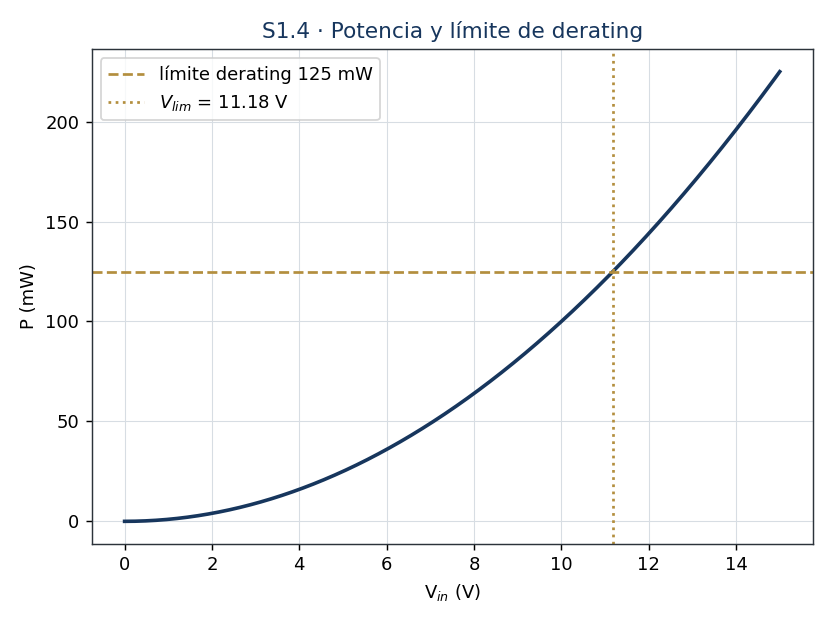
\includegraphics[width=0.78\textwidth]{figs/s14_derating.png}
    \end{center}
    \begin{itemize}
      \item La potencia crece con $V^2$ y cruza el límite de 125 mW en 11.18 V.
    \end{itemize}
  \end{frame}

  % ---------------------------------------------------------------------
  \begin{frame}{Errores comunes}
  \begin{table}
    \small
    \begin{tabular}{p{0.34\textwidth}p{0.30\textwidth}p{0.30\textwidth}}
      \toprule
      Error & Consecuencia & Corrección \\
      \midrule
      Confundir nominal con ``seguro'' & Componente sobrecargado & Aplicar derating de 50\,\% \\
      Calcular con $V_{nominal}$ y no con el peor caso & Límite mal dimensionado & Usar $V_{max}^2/R_{min}$ (WCCA) \\
      Ignorar la temperatura ambiente & Falla térmica prematura & La nominal cae al subir la temperatura \\
      Pensar que ``no se calienta'' a baja corriente & Olvidar $P = V^2/R$ & La potencia depende de la tensión, no solo de la corriente \\
      \bottomrule
    \end{tabular}
  \end{table}
\end{frame}

% ---------------------------------------------------------------------
\begin{frame}{Lectura aeroespacial}
  \begin{itemize}
    \item \textbf{Vacío:} sin convección, el calor solo se evacúa por conducción y
      radiación; el resistor se calienta mucho más rápido que en tierra.
      Se acopla a chasis con planos de cobre y vías térmicas.
    \item \textbf{WCCA:} el peor caso es $P = V_{max}^2/R_{min}$: bus de 32 V con
      resistor de $-1\,\text{\%}$ exige casi el doble de potencia que el caso nominal.
    \item \textbf{Envejecimiento y radiación:} el derating compensa la degradación
      de años en órbita; NASA LLIS-0676 y ECSS-Q-ST-30-11C fijan el 50\,\%.
    \item Un resistor que disipa 56 W con nominal de 60 W ``funciona'' en el papel
      y se \textbf{rechaza}: subir nominal, distribuir o cambiar topología.
  \end{itemize}
\end{frame}

% ---------------------------------------------------------------------
\begin{frame}{Preguntas de verificación}
  \begin{enumerate}
    \item ¿Por qué $P$ crece con el cuadrado de $V$ y no linealmente?
    \item ¿A qué tensión un resistor de \SI{2.2}{\kilo\ohm} / \SI{0.25}{\watt} alcanza el límite de derating?
      \uncover<2->{\emph{($V_{lim}=\sqrt{0.125\cdot 2200}=\SI{16.58}{\volt}$.)}}
    \item ¿Cumple derating un resistor que disipa \SI{0.2}{\watt} con nominal de \SI{0.25}{\watt}?
      \uncover<3->{\emph{(No: $0.2 > 0.125$ W.)}}
    \item ¿Qué cambia si el bus sube de 12 V a 14 V?
      \uncover<4->{\emph{(Disipación +36\,\%: $1.4^2 \approx 1.96$.)}}
    \item ¿Por qué la nominal se reduce al subir la temperatura ambiente?
  \end{enumerate}
\end{frame}


\end{document}
